Consider the symmetric right square pyramid frustum, herein referred to as a right frustum, shown in Figure \ref{fig:p3squareFrustum}. It is composed of a pair of parallel squares centred on the \(z\)-axis joined by four identical trapezia. It has constant uniform magnetisation \(\mathbf{M} = \left[ 0, 0, M_z \right]\) and a relative permeability \(\mu_r\) of unity. The top surface has a side length of \(L\), the bottom surface has a side length of \(l\), and the slanted faces form an angle \(\theta\) with the bottom face. The volume of the frustum is given by
\begin{equation}
V = \frac{l-L}{6}\tan\theta \left( L^2 + lL+ l^2 \right) \text{,}
\end{equation}
and a length parameter\footnote{In this section, \(\upsilon\) is a length based on the volume, and is used to nondimensionalise lengths, allowing a dimensionless analysis.} \(\upsilon\) is defined as \(\upsilon = \sqrt[3]{V}\).

If the field is to be evaluated at any point on the \(z\)-axis, i.e. at a point \(\left(0,0,z\right)\), symmetry can be exploited and the field produced by the magnet can be evaluated with a single function, given by
\begin{figure}
	\centering
	

\begin{subfigure}[t]{\linewidth}

\centering
\tdplotsetmaincoords{70}{45}
\begin{tikzpicture}[scale=0.1,tdplot_main_coords]

% Define coordinates:
\coordinate(ppb) at (20,20,-20);
\coordinate(pnb) at (20,-20,-20);
\coordinate(nnb) at (-20,-20,-20);
\coordinate(npb) at (-20,20,-20);
\coordinate(ppt) at (10,10,0);
\coordinate(pnt) at (10,-10,0);
\coordinate(nnt) at (-10,-10,0);
\coordinate(npt) at (-10,10,0);

% Fill in polygons:
\filldraw[fill=white] (ppt) -- (pnt) -- (nnt) -- (npt) -- cycle;
\filldraw[fill=white] (ppt) -- (ppb) -- (pnb) -- (pnt) -- cycle;
\filldraw[fill=white] (pnt) -- (nnt) -- (nnb) -- (pnb) -- cycle;

% Axes:
\def\lim{13}
\draw[->] (0,0,0) -- (\lim,0,0);
\draw[->] (0,0,0) -- (0,\lim,0);
\draw[->] (0,0,0) -- (0,0,\lim);
\node(xaxis) at (\lim+2,0,0) {\(x\)};
\node(yaxis) at (0,\lim+2,0) {\(y\)};
\node(zaxis) at (0,0,\lim+2) {\(z\)};

\end{tikzpicture}

\subcaption{}
\label{subfig:p3frustum3d}

\end{subfigure}

\vspace{20pt}

\begin{subfigure}[t]{\linewidth}

\centering
\begin{tikzpicture}[scale = 0.2]

\def\LL{5}
\def\ll{10}
\def\hh{10}

% Define coordinates:
\coordinate(tl) at (-\LL,0);
\coordinate(tr) at (\LL,0);
\coordinate(bl) at (-\ll,-\hh);
\coordinate(br) at (\ll,-\hh);

% Draw shape
\draw (tl) -- (tr) -- (br) -- (bl) -- cycle;

% Draw axes
\def\arrowlim{7}
\draw[->] (0,0) -- (\arrowlim,0);
\draw[->] (0,0) -- (0,\arrowlim);
\node(x) at (\arrowlim+1,0) {\(x\)};
\node(z) at (0,\arrowlim+1) {\(z\)};

% Draw dimensions
\def\hoffset{12}
\draw[<->] (\hoffset,0) -- (\hoffset,-\hh);
\node(h) at (\hoffset+1,-5) {\(h\)};
\node(l) at (0,-\hh-1.5) {\(l\)};
\node(L) at (0,-1.5) {\(L\)};
\node(theta) at (-7.5,-8.5) {\(\theta\)};

% Draw an invisible line to centre the figure
\draw[<->,white] (-\hoffset-2,0) -- (-\hoffset-2,-\hh);

% Draw magnetisation vector
\draw[->,thick] (0,-8) -- (0,-4);
\node(M) at (1.5,-6) {\(\mathbf{M}\)};

\end{tikzpicture}

\subcaption{}
\label{subfig:p3frustumschematic}

\end{subfigure}


	\caption{Three-dimensional view (\subref{subfig:p3frustum3d}) and schematic (\subref{subfig:p3frustumschematic}) of a right square pyramid frustum permanent magnet with magnetisation vector \(\mathbf{M}\). The origin is located at the centre of the top surface and both rectangular surfaces are parallel to the \(XY\)-plane. The frustum has a nondimensional height \(h\), a top surface side length \(L\), and bottom surface side length \(l\). The four angled surfaces form an angle \(\theta\) with the bottom surface.}
	\label{fig:p3squareFrustum}
\end{figure}
\begin{align}
B_x = &\ 0 \nonumber \\
B_y = &\ 0 \nonumber \\
B_z = &\ \frac{\mu_0 M_z}{\pi} \left[ \arctan\left(\frac{L^2}{4zR_{0}}\right) - \arctan\left(\frac{l^2}{4\left(z+h\right)R_{1}}\right)\right. \nonumber \\
&\ +\left. \sum_{p=0}^1 \sum_{q=0}^1 \left(-1\right)^{p+q} \cos\theta \Big(\arctan\left(U_{pq}\right) \cos\theta    \Big.\right. \nonumber \\
&\qquad \ \left.\Big.  - \ln\left(T_{pq}\right)\sin\theta - \frac{\left(-1\right)^p\sin\theta}{\sqrt{1+\sec^2\theta}} \ln\left({S_{pq}}\right) \Big) \right] \text{,}
\end{align}
where
\begin{align*}
l_q &= L + 2hq\cot\theta \\
R_{q} &= \sqrt{\frac{l_q^2}{2}+\left(z+qh\right)^2} \\
S_{pq} &= l_q\cos\theta + \left(z+qh\right)\sin\theta + \sqrt{1+\cos^2\theta}R_{q} \\
T_{pq} &= R_{q} - \frac{\left(-1\right)^p l_q}{2} \\
U_{pq} &= \frac{\left(-1\right)^p\left(z+qh\right)}{R_{q}} \text{.}
\end{align*}
It should be noted that a cylindrical frustum can produce a stronger field than that of a rectangular frustum along the axis of symmetry. However, rectangular frusta have the ability to tessellate well (as discussed in Section \ref{sec:p3planarArray}), and as such only rectangular frusta are considered in this work.

A right frustum requires three parameters to fully describe the geometry. For a magnet with a given volume \(V\), the length dimensions can be normalised by the length parameter \(\upsilon\). Here, the normalised height \(h/\upsilon\) and wall angle \(\theta\) are varied for a frustum with volume \(V\). For each pair \((h/\upsilon,\theta)\), the magnetic field produced by the frustum was evaluated at the point \(\left( 0, 0, z/\upsilon\right)\) and normalised by the magnetisation strength of the magnet.

First, the field was evaluated at \(z/\upsilon = 0.1\) for all physically realisable pairs \(\left( h/\upsilon, \theta\right)\), where physically realisable refers to all lengths being positive and real, and a contour plot drawn in Figure \ref{subfig:p3centralField100}. The field is maximised by a frustum with a normalised height of \(h_\text{opt}/\upsilon = 0.95\) units and a wall angle of \(\theta_\text{opt} =\) \ang{57}. The equivalent optimal cuboidal magnet is found in the same way, but constraining the wall angle to \ang{90}. For \(z/\upsilon = 0.1\), the optimal frustum produces a field 12.6\% stronger than the optimal cuboid. Schematics of both the optimal frustum and optimal cuboid for \(z/\upsilon = 0.1\) are shown in Figure \ref{fig:p3optimalGeom_z_0_1}. This optimisation was repeated for a point \(z/\upsilon = 0.5\) units above the magnet (Figure \ref{subfig:p3centralField500}), resulting in an optimal frustum with \(h_\text{opt}/\upsilon = 0.83\) units and \(\theta_\text{opt} =\) \ang{94}. This optimal frustum is almost cuboidal in shape, leading to a field only 0.07\% stronger than the equivalent optimal cuboid.

To give an indication of optimal magnet shape, the \(z\)-field was calculated in the region above a cube magnet, shown in Figure \ref{fig:p3optimalFrusAndCube}. In addition, the optimal cuboid and frustum for \(z/\upsilon = 0.1\) were drawn, with a `+' sign representing the point at which the field is maximised. All three magnets have identical volumes and magnetisations, with the field calculated over the same region; only the shape of the magnet differs. It can be seen that the cube magnet has the weakest field strength at this point, with the optimal cuboid having a slightly stronger field. However, the optimal frustum `focuses' the flux through the top surface, leading to a larger magnetic field at the point of interest.
\begin{figure}
    \centering
	\begin{subfigure}{0.8\textwidth}
		\centering
		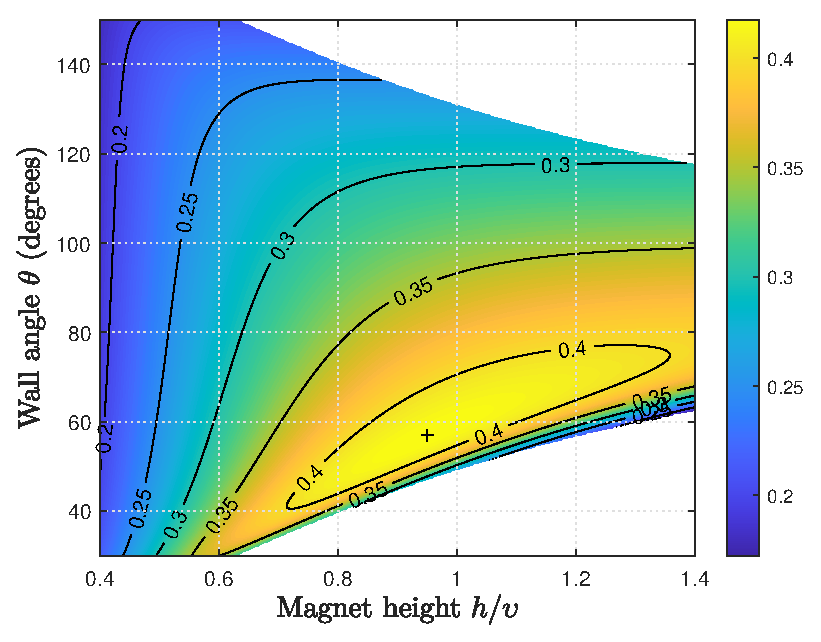
\includegraphics[width=\linewidth]{p3/p3FIG5a}
		\subcaption{}
		\label{subfig:p3centralField100}
	\end{subfigure}
	
	\begin{subfigure}{0.8\textwidth}
		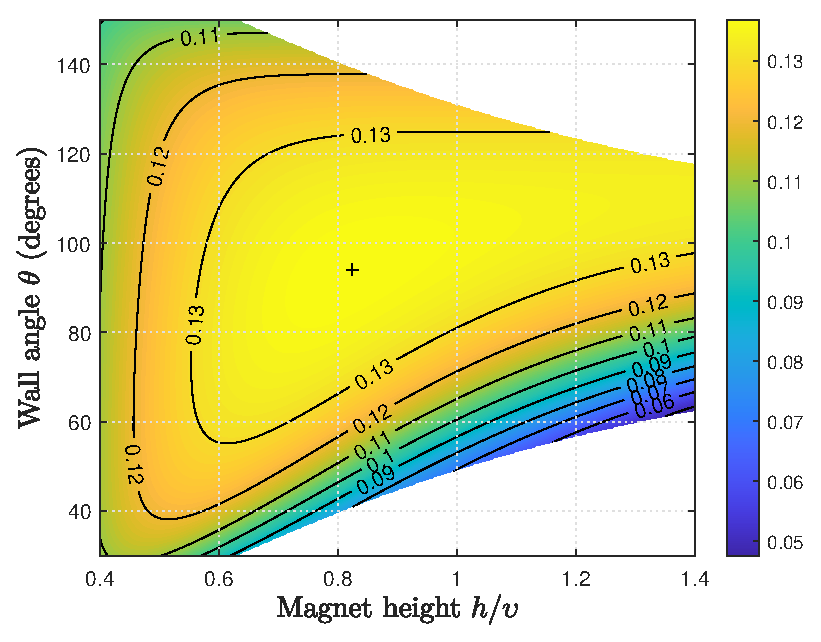
\includegraphics[width=\linewidth]{p3/p3FIG5b}
		\subcaption{}
		\label{subfig:p3centralField500}
	\end{subfigure}
	\caption{Normalised magnetic field strength \(z/\upsilon = 0.1\) (\subref{subfig:p3centralField100}) and \(z/\upsilon = 0.5\) (\subref{subfig:p3centralField500}) units above the centre of a right frustum magnet with a volume \(V\), a normalised height of \(h/\upsilon\) units and wall angle of \(\theta\) degrees. The global maxima \(\left( h_\text{opt}/\upsilon, \theta_\text{opt}\right)\) for each plot is highlighted with a `+', with the white regions indicating non-physical geometries.}
	\label{fig:p3centralField}
\end{figure}
\begin{figure}
	\centering
	

\begin{subfigure}[t]{0.45\linewidth}

\centering
\begin{tikzpicture}[scale = 0.3]

\def\LL{1}
\def\ll{4.5950}
\def\hh{5.5312}

% Define coordinates:
\coordinate(tl) at (-\LL,0);
\coordinate(tr) at (\LL,0);
\coordinate(bl) at (-\ll,-\hh);
\coordinate(br) at (\ll,-\hh);

% Draw shape
\draw (tl) -- (tr) -- (br) -- (bl) -- cycle;

% Draw dimensions
\def\hoffset{6}
\draw[<->] (-\hoffset,0) -- (-\hoffset,-\hh);
\node(h) at (-\hoffset-1.5,-2.7656) {0.951};
\draw[<->] (-\ll,-\hh-1.5) -- (\ll,-\hh-1.5);
\node(l) at (0,-\hh-2.5) {1.580};
\draw[<->] (-\LL,1.5) -- (\LL,1.5);
\node(L) at (0,2.5) {0.344};

\end{tikzpicture}

\subcaption{}
%\label{subfig:frustumschematic}

\end{subfigure}
~ \hfill ~
\begin{subfigure}[t]{0.45\linewidth}

\centering
\begin{tikzpicture}[scale = 0.3]
	
\def\LL{2.3647}
\def\ll{2.3647}
\def\hh{8.8066}

% Define coordinates:
\coordinate(tl) at (-\LL,0);
\coordinate(tr) at (\LL,0);
\coordinate(bl) at (-\ll,-\hh);
\coordinate(br) at (\ll,-\hh);

% Draw shape
\draw (tl) -- (tr) -- (br) -- (bl) -- cycle;

% Draw dimensions
\def\hoffset{5}
\draw[<->] (\hoffset,0) -- (\hoffset,-\hh);
\node(h) at (\hoffset+1.5,-4.4033) {1.514};
\draw[<->] (-\ll,-\hh-1.5) -- (\ll,-\hh-1.5);
\node(l) at (0,-\hh-2.5) {0.813};

% Draw an invisible line to centre the figure
%\draw[<->,white] (-\hoffset-2,0) -- (-\hoffset-2,-\hh);

\end{tikzpicture}

\subcaption{}
%\label{subfig:frustumschematic}

\end{subfigure}


	\caption{Normalised dimensions of the optimal frustum (left) and cuboid (right) to maximise the field for \(z/\upsilon = 0.1\). Both magnets have identical volume, but the optimal frustum has a smaller top face, which `focuses' flux, giving a slightly stronger field in the small region above the centre of the magnet.}
	\label{fig:p3optimalGeom_z_0_1}
\end{figure}
\begin{figure*}
	\centering
	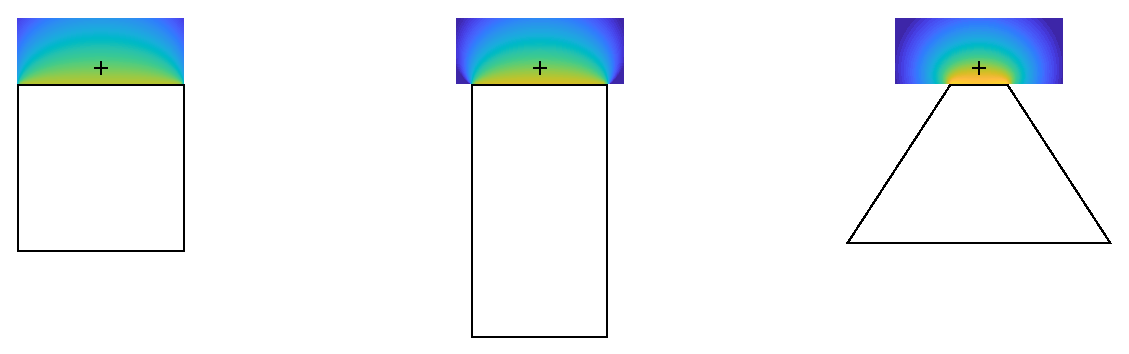
\includegraphics[width=\linewidth]{p3/p3FIG7}
	\caption{The \(z\)-field in the region above a cube magnet, the optimal cuboid magnet, and the optimal frustum magnet for \(z/\upsilon = 0.1\). The point \(z/\upsilon = 0.1\) is drawn with a `+', showing that the optimal frustum magnet gives the strongest field at this point.}
	\label{fig:p3optimalFrusAndCube}
\end{figure*}

An interior-point optimisation algorithm was used to calculate the optimal frustum geometry for a large range of distances \(z/\upsilon\) above the magnet. The optimal parameters \(h_\text{opt}/\upsilon\) and \(\theta_\text{opt}\) were calculated at each \(z/\upsilon\) and are plotted in Figure \ref{fig:p3optimalFrustumGeometry}. As \(z/\upsilon\) increases, the optimal height \(h_\text{opt}/\upsilon\) shows a decreasing trend and the wall angle \(\theta_\text{opt}\) shows an increasing trend. Interestingly, the optimal height \(h_\text{opt}/\upsilon < 1\) for all values of \(z/\upsilon\), meaning the optimal geometry is always a `flatter' magnet. The magnetic field strength for both optimal frustum and optimal cuboid are plotted in Figure \ref{fig:p3PFIeps}, along with the percentage increase in field strength using the optimal frustum rather than the optimal cuboid. This shows a negligible increase in field strength for large \(z/\upsilon\). However, for small \(z/\upsilon\), the increase in field strength may allow more effective use in applications such as magnetic power transmission, linear vibrating systems, and magnetic latching.
\begin{figure}
	\centering
	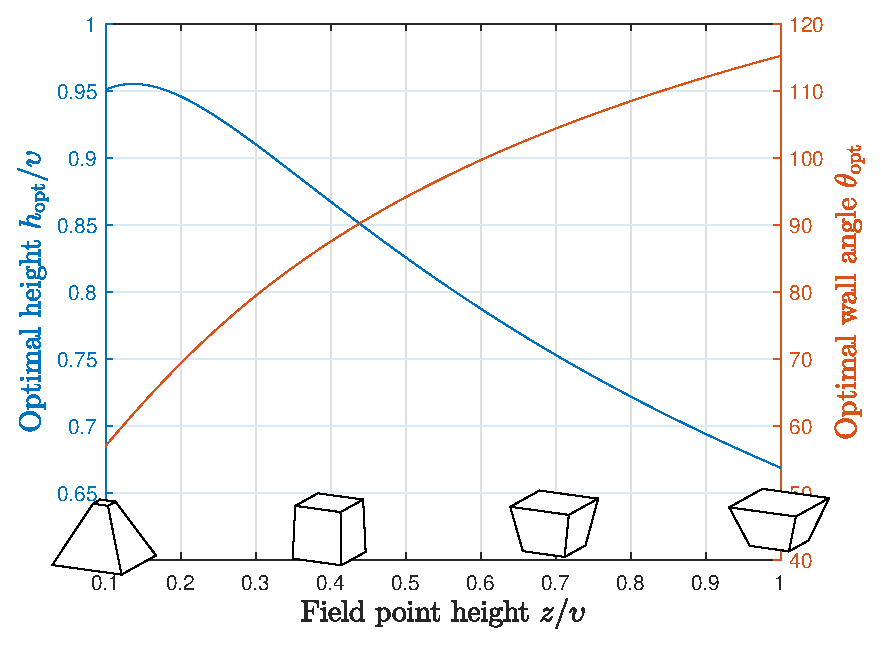
\includegraphics[width=0.8\textwidth]{p3/p3FIG8}
	\caption{Optimal frustum height \(h_\text{opt}\) (blue) and wall angle \(\theta_\text{opt}\) (orange) to maximise the magnetic field strength a distance \(z/\upsilon\) above a right frustum permanent magnet with a volume of \(V\) units\(^3\). A small image of the optimal frustum geometry is displayed at the bottom of the figure for the values \(z/\upsilon =\ \)0.1, 0.4, 0.7, and 1.0.}
	\label{fig:p3optimalFrustumGeometry}
\end{figure}
\begin{figure}
	\centering
	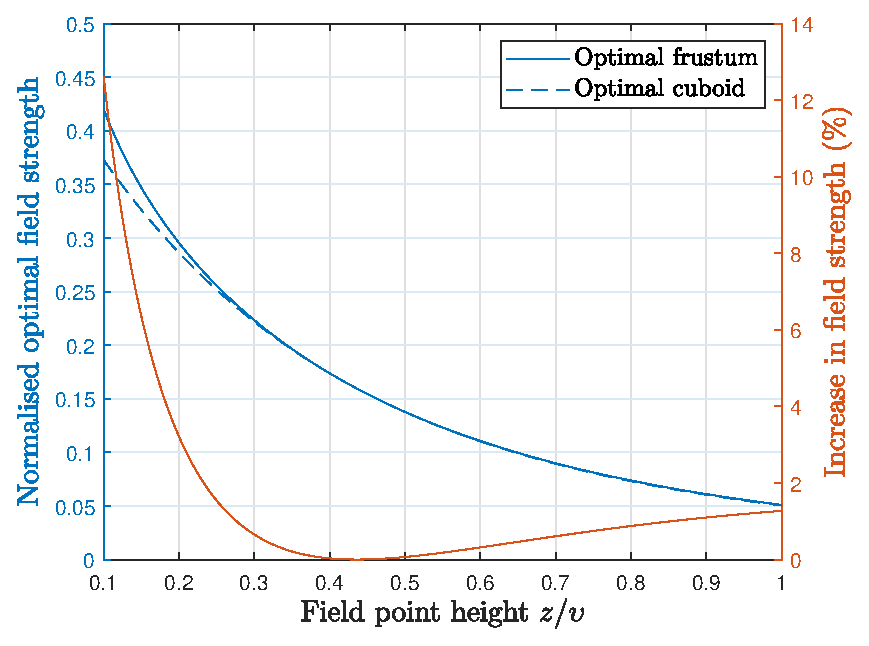
\includegraphics[width=0.8\textwidth]{p3/p3FIG9}
	\caption{Magnetic field strength produced by an optimal frustum and cuboid of the same volume (blue) and percentage increase in the field strength produced by the frustum over the cuboid (orange).}
	\label{fig:p3PFIeps}
\end{figure}